\section{Bibliography Review}
\label{sec:bibliography-review}

A bibliographical research was performed to determine the state of the art in the field of the project,
both in terms of the models and algorithms used as well as the chosen and best performing state and action spaces,
with regard to realistic environment simulations, and the use of reinforcement learning techniques.
The search was made using the ``Web of Science'' repository <cite>, covering the last 5 years, with the following search key:

\begin{verbatim}
    ("reinforcement learning" OR "dynamic programming" OR
     "optimal control" OR "control theory" OR "machine learning")
    AND
    ("market making" OR "market maker")
\end{verbatim}

Initially, 64 references were selected and deemed relevant to the project,
with 23 of them being selected for further analysis and effectively used in our analysis,
with 4 of them being added to the list after the initial selection.
The references were selected based on their relevance to the project,
and tagged according to the following groups (for each non-binary category, combination of tags were allowed):
type of data (if simulated or on real-time connections);
choosen state space (tensors of bid-ask spreads, order imbalance, and even N-depth order book);
choosen action space (limit orders, market orders, and others);
reward space (spread, volume, profit, and others);
algorithms used (Q-Learning, Deep Q-Learning, Actor-Critic, or others);
if using a multi-agent approach or not (Dueling or Market Agents); and the use of model-free environments;
finally, we also tagged the results by choosen metrics (Sharpe Ratio, PnL, and others);
and by benchmarking results (against other models or strategies).

\subsection{State, Action, and Reward Spaces}

% Choosen State Space
% State variable
% Total times used
%{
%    "inventory": "Agent inventory",
%    "bidask spread": "Bid-Ask spread",
%    "lob": "Price Levels",
%    "midprice": "Midprice",
%    "order status": "Posted order status",
%    "volume": "Transaction volume",
%    "order imbalance": "Order imbalance",
%    "volatility": "Volatility",
%    "price prediction": "Price prediction",
%    "time": "Market time"
%}

% graph: images/state_space.png
\begin{figure}[H]
    \centering
    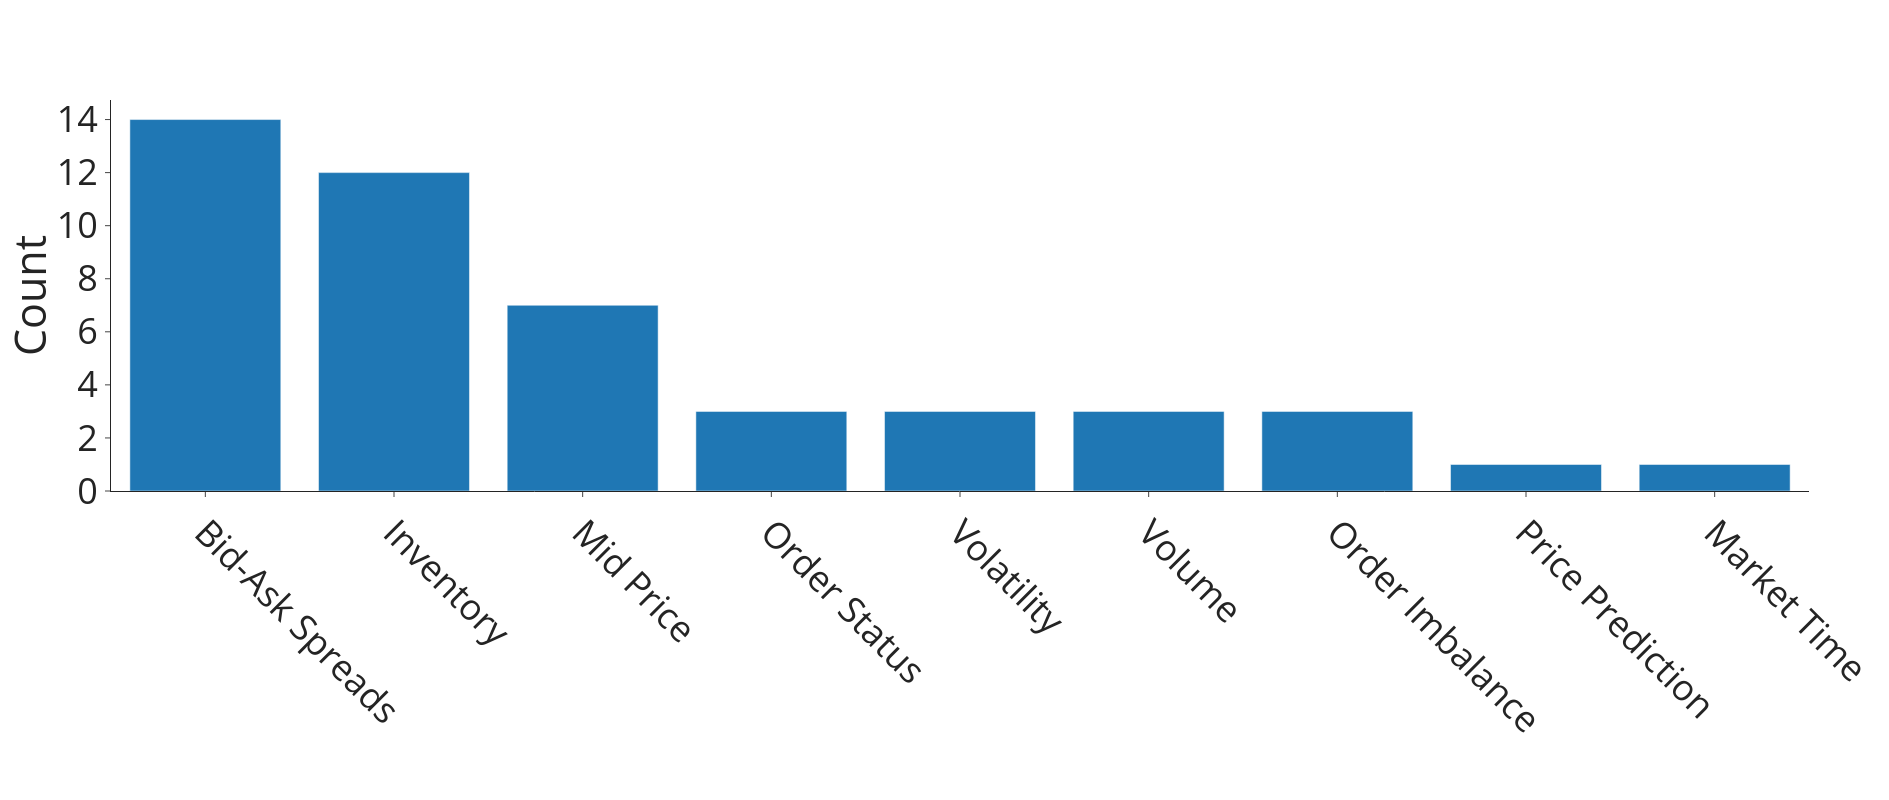
\includegraphics[width=0.8\textwidth]{images/state_space}
    \caption{State Space}
    \label{fig:state-space}
\end{figure}